\section{Problem 2B: Stochastic SIR model}

\subsection{a)}

As seen in the plot in figure \ref{fig:SIR_stoch}, the $10$ different realisations of the stochastic SIR model , shown in dashed lines in graded colours, seem to lie close to the deterministic solution.

\begin{figure}[htb]
	\centering
	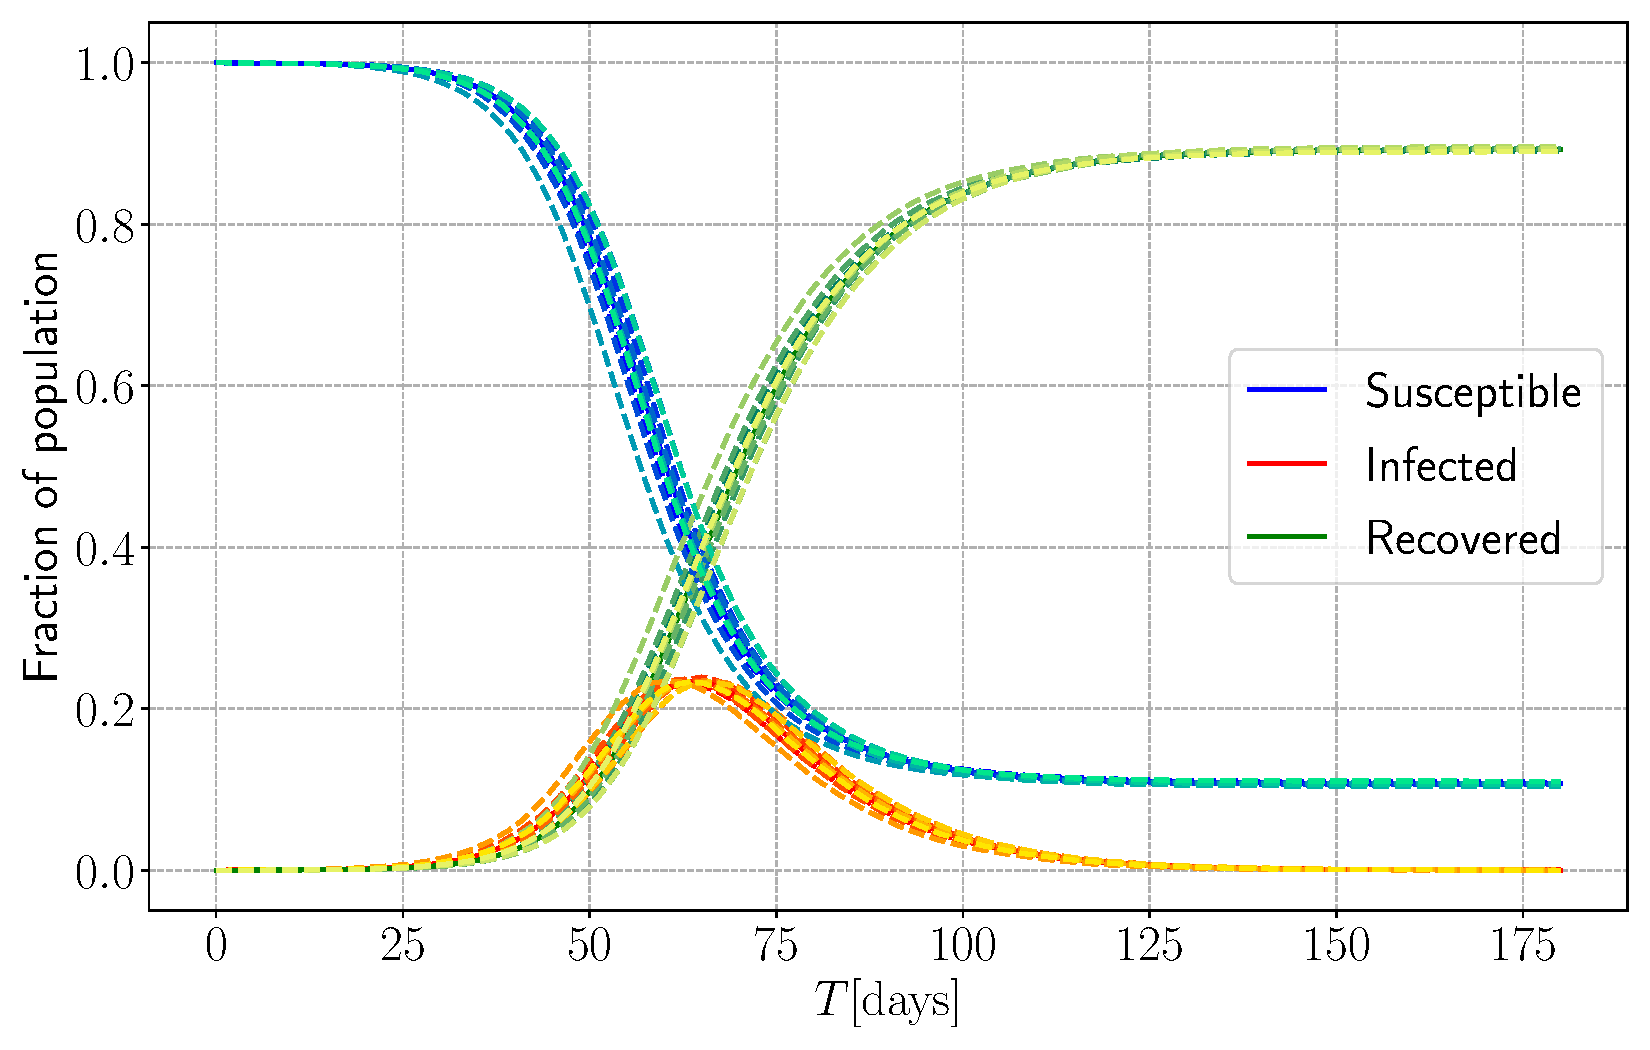
\includegraphics[width=0.8\columnwidth]{../fig/2Ba_SIR.pdf}
	\caption{Solution of stochastic SIR equations with $\beta = 0.25\, \mathrm{day}^{-1}$, $\tau = 10\, \mathrm{day}$.}
	\label{fig:SIR_stoch}
\end{figure}

To choose a suitable time-step for simulating this model, I run the simulation up to $t = 10$ days and find the deviation between the fraction of infected people with the semi-analytical result for the early stages given by equation \ref{eq:Iexp}. I compute this using the average of $200$ runs of the stochastic model. I include the same run with the deterministic model to see how the deviations relate to each other. This is shown in figure \ref{fig:timesteps}. Clearly, using this comparison is \textit{not} a good way of determining the time step we want to use for the deterministic model, as the solution approaches the reference values very quickly for the chosen step lengths. The stagnation observed here is probably due to the fact that the reference solution is an approximation itself! However, we see from this plot that if we choose a step length $\lesssim 0.01$, the deviations of the stochastic solution start to flatten out, and become smaller than $10^{-5}$, which is the highest accuracy we can expect to get when using $100\,000$ people in the population for the stochastic model (i.e. less than one person difference in the fraction of infected). I therefore always use a time step smaller than $0.01$ for simulating the stochastic models. In particular, I use $\Delta t = 0.005$ in problem B,C,D and Ea. For Eb I use $\Delta t = 0.01$ because the runtime becomes uncomfortably large when using smaller time steps.

For determining the step length to use for the deterministic model I create a reference solution using a relatively small time step, $\Delta t = 10^{-4}$, and then use the deviations between this and each run at the endpoint as a measure of the absolute error. After having done that, it is mostly a matter of preference how small a step length one wants to use. If I can accept an error of $10^{-8}$ in the fraction of susceptible after $50$ days --- corresponding to $1/1000$ of an individual --- I see from the plot in figure \ref{fig:timesteps_det} that I will have to use $\Delta t \lesssim 10^{-1}$. Since the runtimes of the simulation for $\Delta t < 10^{-2}$ for $50$ days are always less than $1$ second, I find that $\Delta t = 0.005$ is probably more than sufficient, and appropriate considering both runtime and accuracy.    
\begin{figure}[htb]
\centering
\begin{minipage}[c]{0.49\columnwidth}
	\centering
	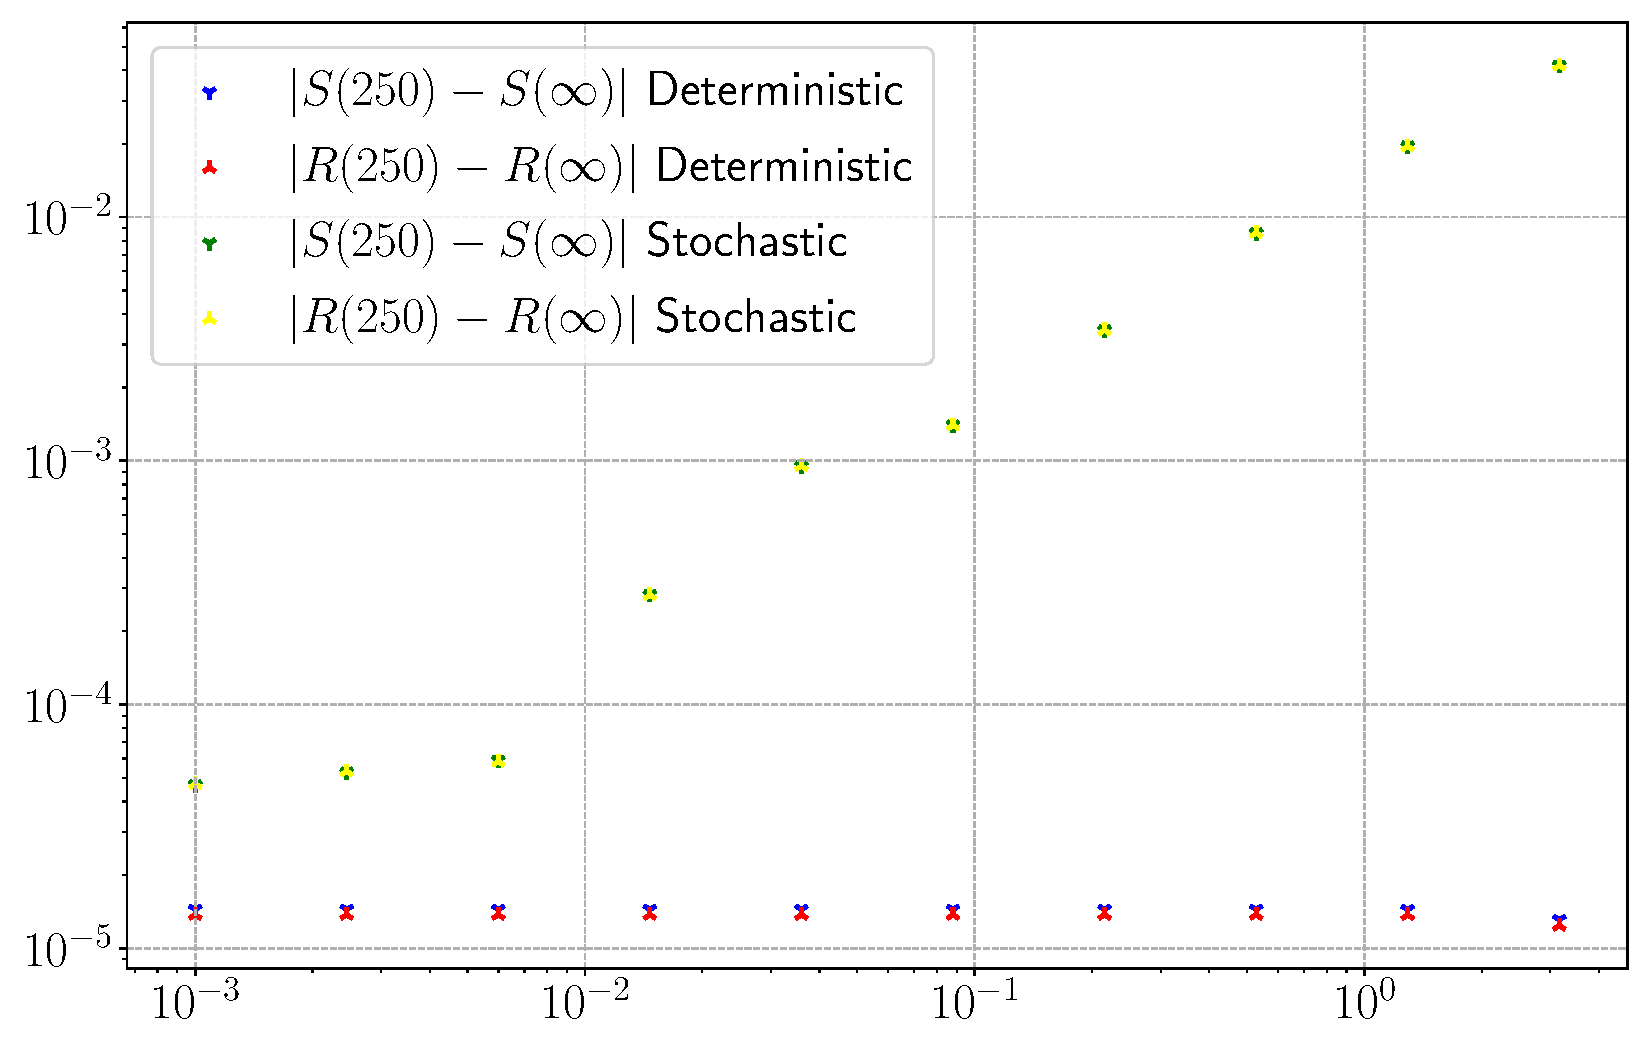
\includegraphics[width=\columnwidth]{../fig/timestep.pdf}
	\captionof{figure}{Global error for stochastic model, using the analytical expression for short times, $I_{\mathrm{ref}}$, as reference.}
	\label{fig:timesteps}
\end{minipage}
\hfill
\begin{minipage}[c]{0.49\columnwidth}
	\centering
	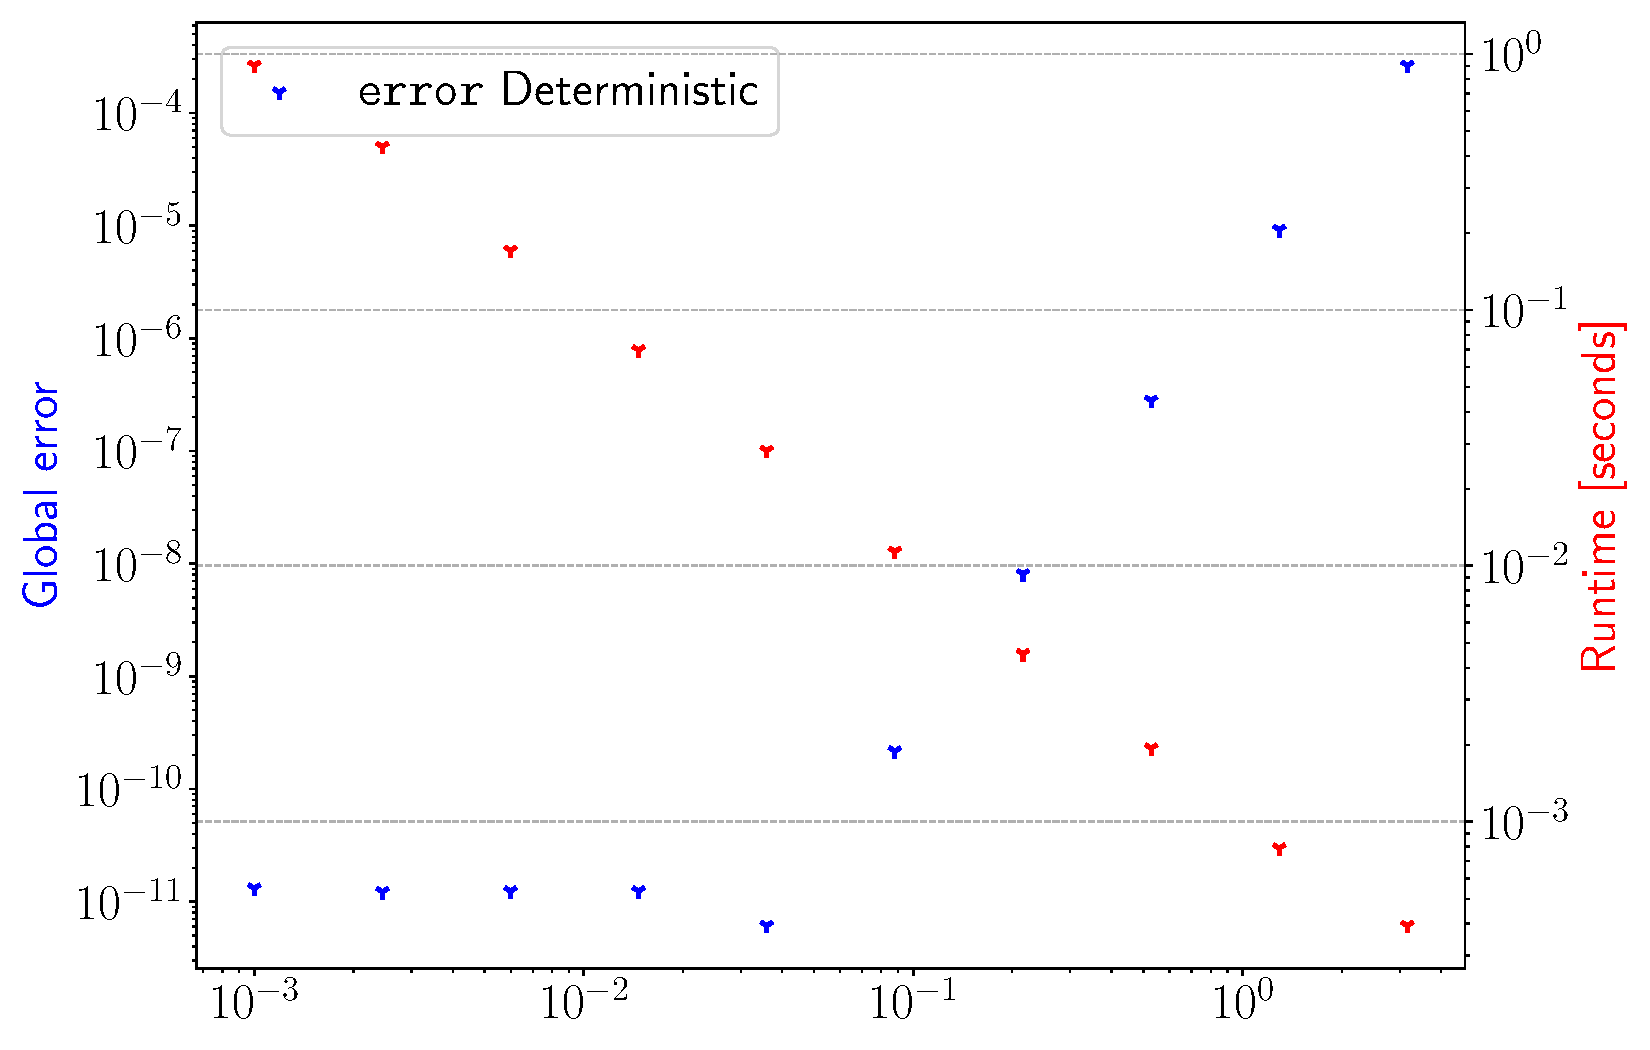
\includegraphics[width=\columnwidth]{../fig/timestep_det.pdf}
	\captionof{figure}{Global error the deterministic model, using a simulation with $\Delta t = 10^{-4}$ as reference. }
	\label{fig:timesteps_det}
\end{minipage}
\end{figure}
\subsection{b)}
As in the previous exercise, we plot the fraction of infected people together with the analytical model for the early stages. This is shown in figure \ref{fig:Infected_stoch}. Here we clearly see that all the realisations are approximately linear in the semi-log plot in the first $40$ days, or so, of the simulation as we observed in the previous exercise. The mean slope of the $10$ realisations is shown in table \ref{tab:2Bb} together with the standard deviation. This is reasonably close to the expected value, which is $\beta - 1/\tau = 0.15$. 
\begin{figure}[htb]
	\centering
	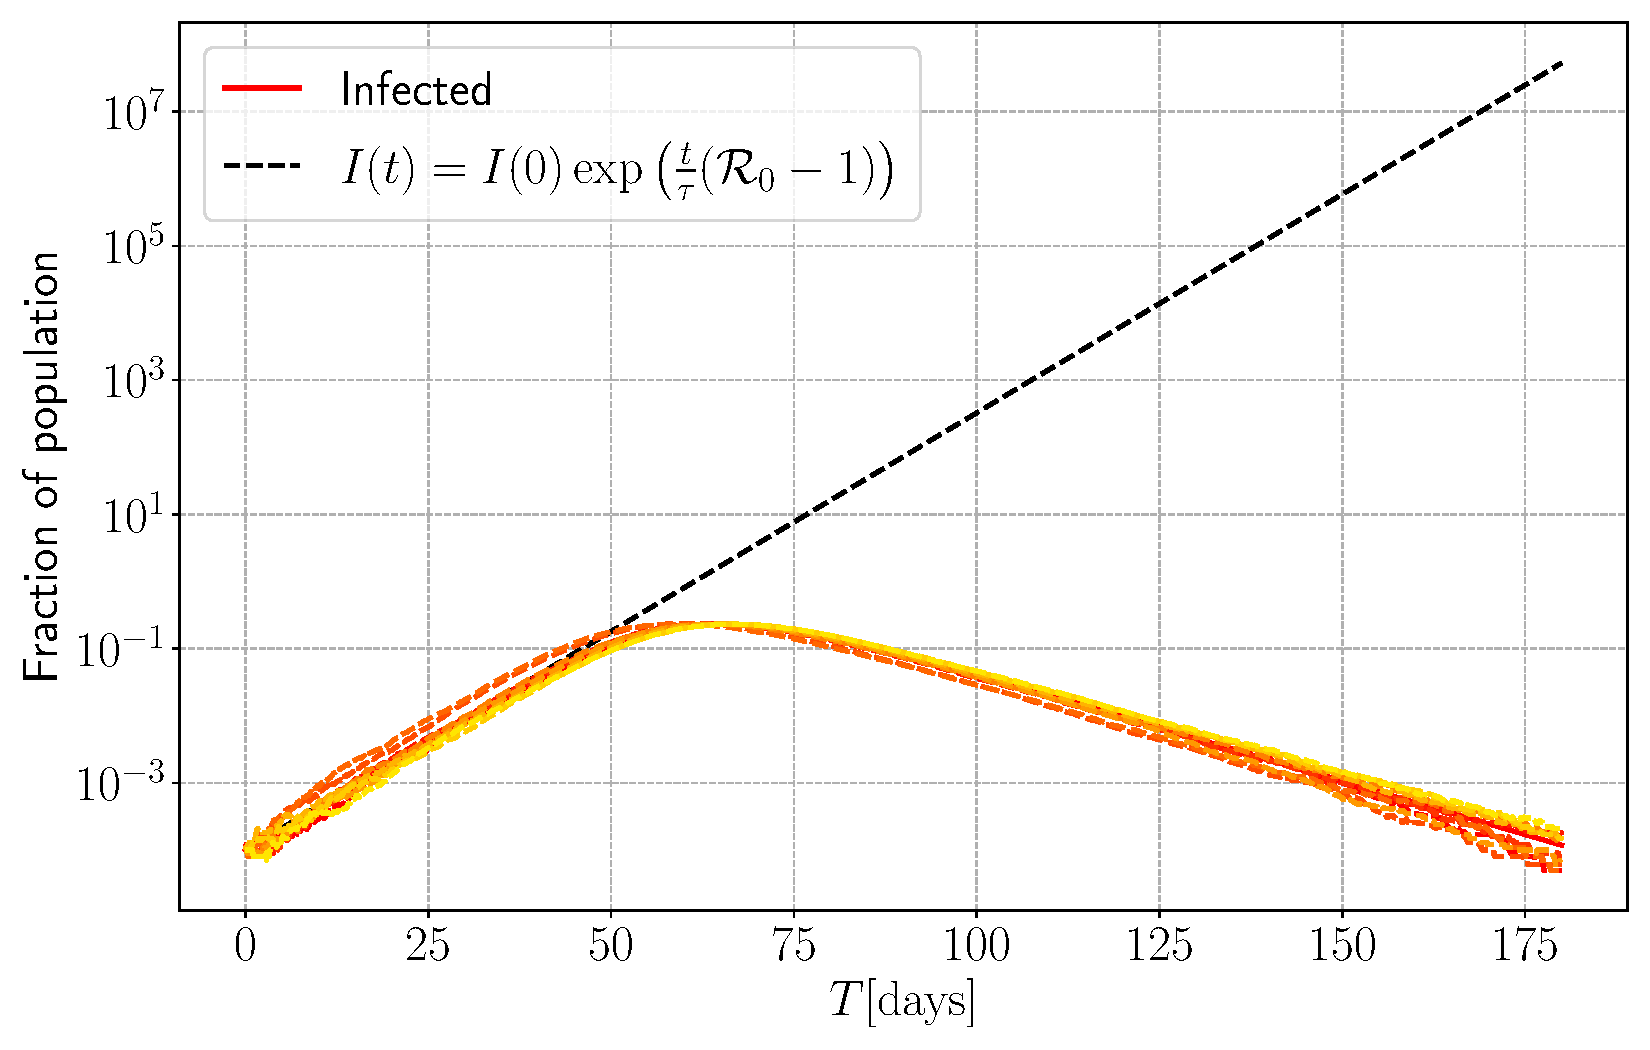
\includegraphics[width=0.8\columnwidth]{../fig/2Bb_I.pdf}
	\caption{Infected people compared with the analytical approximation at the early stages. Stochastic and deterministic model.}
	\label{fig:Infected_stoch}
\end{figure}
\begin{table}[htb]
	\centering
	\caption{Mean slope of the $10$ realisation shown in figure \ref{fig:Infected_stoch} and standard deviation.}
	\begin{tabular}{cc}%
	    \toprule 
	    \bfseries Initial log slope & \bfseries Standard deviation 
	    \csvreader[head to column names]{../data/slopes.csv}{}% use head of csv as column names
	    {\\ \Logslope & \Deviation }\\
		\bottomrule
	\end{tabular}
	\label{tab:2Bb}
\end{table}
\newpage

\subsection{c) Probability of an outbreak}

There will always be a certain probability for an outbreak disappearing by itself using the stochastic model. In the present subsection we estimate this probability for an initial number of infected people $=1,2,\dots,10$. This is done by the procedure described in algorithm \ref{alg:prob_I}. In this procedure, I use the slope of the number of infected people $I(t)$ during the first $30$ days as an indicator of whether the outbreak disappears by itself or not. If the slope is positive, I count it as an outbreak, and if not, I count it as disappearing.

\begin{algorithm}[H]
	Choose the parameters of the model as those given in the exam sheet \cite{sheet}, but with $T = 30 \, \mathrm{days}$\footnote{As the typical infection time is $10$ days, I assume 30 days to be sufficient for detecting an outbreak in the stochastic model.}. \;
	Choose a batch-size $B$.\;
	\For{$I = 1,2,\dots, 10$}{
		Initialise an empty vector of length $B$: $\mathbf{X} = [0,\dots,0]$.\;
		\For{$n = 1,\dots, B$}
			{
			Run the simulation with initial number of infected people $= I$.\;
			Calculate the \texttt{slope} in the semi-log axes for $I(t)$.\;
			\eIf{$\texttt{slope} <= 0$}
			{$X_n = 0$}
			{$X_n = 1$}
		}
		Estimate the probability of an outbreak for $I$ initially infected by
		$$
				p \coloneqq P(\mathrm{outbreak}|I) = \frac{1}{B} \sum_{n= 1}^{B} X_n. \;
		$$	
		Calculate the standard deviation of the estimate by 
		\begin{equation}\label{eq:std}
			\sqrt{\mathrm{Var}(\hat{p})} = \sqrt{\frac{p(1-p)}{B}}.
		\end{equation}
	}
	\caption{Calculating the probability of an outbreak as a function of the initial number of infected people, $I$. }
	\label{alg:prob_I}
\end{algorithm} 

In performing this procedure, I use a batch size of $500$ in each sweep. What we are estimating here is essentially a Bernoulli-distributed random variable, $X$: $X$ can take the realisations $1$ or $0$ with probabilities $p$ and $1-p$ respectively, and we assume all the $X_n$s to be independent \cite[~p.26]{Wassermann}. Then, as the variance of such a random variable is $p(1-p)$, the variance of the estimator for the probability, namely $\hat{p}$\footnote{That is, the mean value of $X_n$.}, is 
$$
	\mathrm{Var}(\hat{p}) =  \sum_{n= 1}^{B} \mathrm{Var}\left(\frac{X_n}{B}\right) = \frac{1}{B^2} \sum_{n= 1}^{B} \mathrm{Var}(X_n) = \frac{1}{B^2} \sum_{n= 1}^{B} p (1-p) = \frac{p(1-p)}{B},
$$
from which formula \eqref{eq:std} follows. 

The probability of an outbreak as a function of the initial number of infected people are shown in figure \ref{fig:prob_outbreak} together with the associated standard deviation. As seen from this plot, when there are more than $6$ people initially infected, the probability is approximately $1$ that an outbreak will grow. However, for e.g. $1$ initially infected person, the probability is approximately $0.638 \pm 0.021$. This ultimately shows that the stochastic model has a more realistic feature to it than the deterministic one, in the sense that these scenarios might occur.
% The probabilities are also shown in table \ref{tab: probabilities}

\begin{figure}[htb]
	\centering
	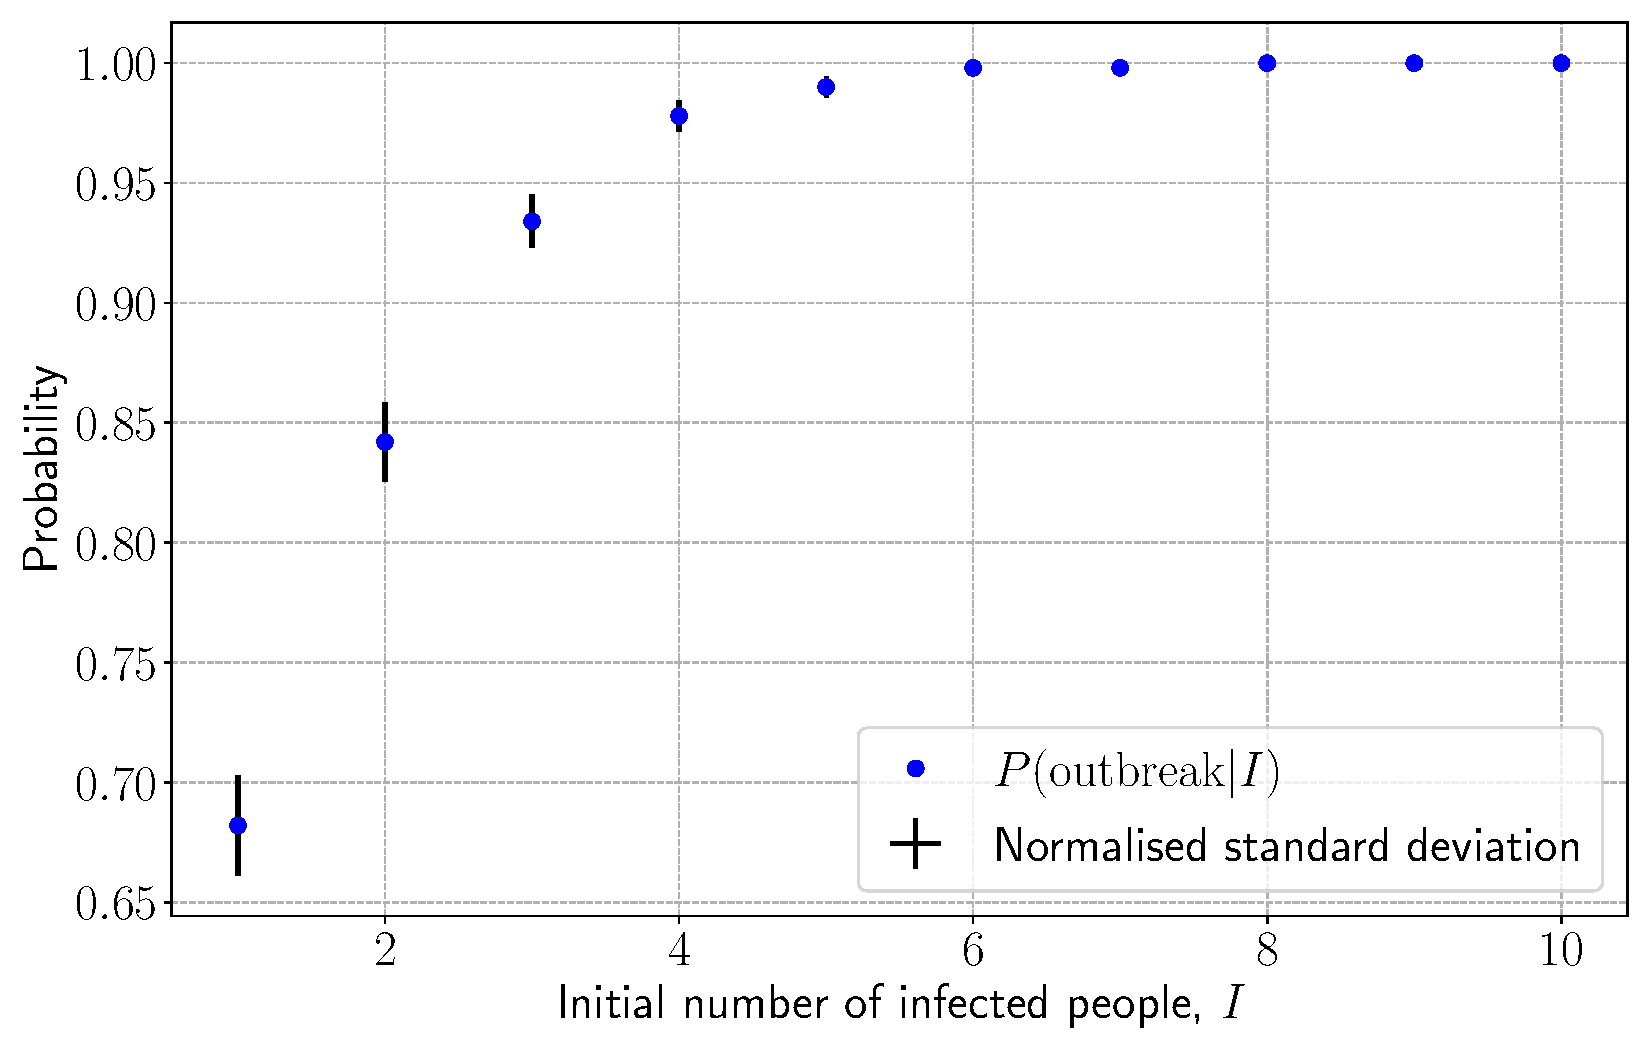
\includegraphics[width=0.8\columnwidth]{../fig/2Bc_prob.pdf}
	\caption{Probability of an outbreak as a function of initial number of infected people.}
	\label{fig:prob_outbreak}
\end{figure}

\clearpage